\documentclass[a4paper]{article}
\usepackage{times}
\usepackage[utf8]{inputenc}
\usepackage[T1]{fontenc}
\usepackage{selinput}
\usepackage{upquote}
\usepackage[margin=2cm, rmargin=4cm, tmargin=3cm]{geometry}
\usepackage{tcolorbox}
\tcbuselibrary{breakable}
\usepackage{xspace}
\usepackage{amsmath}
\usepackage{float}
\usepackage[french]{babel}
\usepackage{hyperref}
\usepackage{xurl}
\usepackage{fontawesome6}
\usepackage{enumitem}
\usepackage{marginnote}
\usepackage{ulem}
\usepackage[yyyymmdd,hhmmss]{datetime}
\usepackage{ulem}
\usepackage{environ}
\usepackage{graphicx}
%\usepackage[top=Bcm, bottom=Hcm, outer=Ccm, inner=Acm, heightrounded, marginparwidth=Ecm, marginparsep=Dcm]{geometry}
\usepackage{courier}



\newtcolorbox{Example}[1]{colback=white,left=20pt,colframe=slideblue,fonttitle=\bfseries,title=#1}
\newtcolorbox{Solutions}[1]{breakable,colback=white,left=20pt,colframe=green,fonttitle=\bfseries,title=#1}
\newtcolorbox{Conseils}[1]{colback=white,left=20pt,colframe=slideblue,fonttitle=\bfseries,title=#1}
\newtcolorbox{Warning}[1]{colback=white,left=20pt,colframe=warning,fonttitle=\bfseries,title=#1}
\newtcolorbox{Note}[1]{colback=white,left=20pt,colframe=grey,fonttitle=\bfseries,title=#1}
\newtcolorbox{Dessin}[1]{colback=white,left=20pt,colframe=grey,fonttitle=\bfseries,title=#1}

\setlength\parindent{0pt}

  %Exercice environment
  \newcounter{exercice}
  \newenvironment{Exercice}[1][]
  {
  \par
  \stepcounter{exercice}\textbf{Question \arabic{exercice}:} (\faClock \enskip \textit{#1})
  }
  {\bigskip}
  

% Title
\newcommand{\titre}{\begin{center}
  \section*{Algorithmes et Pensée Computationnelle}
\end{center}}
\newcommand{\cours}[1]
{\begin{center} 
  \textit{#1}\\
\end{center}
  }



% \newcommand{\exemple}[1]{\newline~\textbf{Exemple :} #1}
\newcommand{\todo}[1]{\textcolor{red}{#1}}
%\newcommand{\attention}[1]{\newline\faExclamationTriangle~\textbf{Attention :} #1}

% Documentation url (escape \# in the TP document)
\newcommand{\documentation}[1]{\faBookOpen~Documentation : \href{#1}{#1}}

% Clef API
\newcommand{\apikey}[1]{\faKey~Clé API : \lstinline{#1}}
\newcommand{\apiendpoint}[1]{\faGlobe~Url de base de l'API \href{#1}{#1}}

%Listing Python style
\usepackage{color}
\definecolor{slideblue}{RGB}{33,131,189}
\definecolor{green}{RGB}{0,190,100}
\definecolor{blue}{RGB}{121,142,213}
\definecolor{grey}{RGB}{120,120,120}
\definecolor{warning}{RGB}{235,186,1}

\usepackage{listings}
\lstdefinelanguage{texte}{
    keywordstyle=\color{black},
    numbers=none,
    frame=none,
    literate=
           {é}{{\'e}}1
           {è}{{\`e}}1
           {ê}{{\^e}}1
           {à}{{\`a}}1
           {â}{{\^a}}1
           {ù}{{\`u}}1
           {ü}{{\"u}}1
           {î}{{\^i}}1
           {ï}{{\"i}}1
           {ë}{{\"e}}1
           {Ç}{{\,C}}1
           {ç}{{\,c}}1
           {ô}{{\^o}}1,
    columns=fullflexible,keepspaces,
	breaklines=true,
	breakatwhitespace=true,
}
\lstset{
  language=Python,
	%basicstyle=\bfseries\footnotesize,
  basicstyle=\footnotesize\ttfamily\small,
	breaklines=true,
	breakatwhitespace=true,
	commentstyle=\color{grey},
	stringstyle=\color{slideblue},
  keywordstyle=\color{slideblue},
	morekeywords={with, as, True, False, Fraction, Float, join, index, None, main, argparse, self, sort, __eq__, __add__, __mul__ ,__ne__, __radd__, __del__, __ge__, __gt__, split, os, endswith, is_file, scandir, @classmethod, this},
	deletekeywords={id},
	showspaces=false,
	showstringspaces=false,
	columns=fullflexible,keepspaces,
	literate=
           {é}{{\'e}}1
           {è}{{\`e}}1
           {ê}{{\^e}}1
           {à}{{\`a}}1
           {â}{{\^a}}1
           {ù}{{\`u}}1
           {ü}{{\"u}}1
           {î}{{\^i}}1
           {ï}{{\"i}}1
           {ë}{{\"e}}1
           {Ç}{{\,C}}1
           {ç}{{\,c}}1
           {ô}{{\^o}}1,
    numbers=left,
}

\newtcbox{\mybox}{nobeforeafter,colframe=white,colback=slideblue,boxrule=0.5pt,arc=1.5pt, boxsep=0pt,left=2pt,right=2pt,top=2pt,bottom=2pt,tcbox raise base}
\newcommand{\projet}{\mybox{\textcolor{white}{\small projet}}\xspace}
\newcommand{\optionnel}{\mybox{\textcolor{white}{\small Optionnel}}\xspace}
\newcommand{\advanced}{\mybox{\textcolor{white}{\small Pour aller plus loin}}\xspace}
\newcommand{\auto}{\mybox{\textcolor{white}{\small Auto-évaluation}}\xspace}


\usepackage{environ}
\newif\ifShowSolution
\NewEnviron{solution}{
  \ifShowSolution
	\begin{Solutions}{\faTerminal \enskip Solution}
		\BODY
	\end{Solutions}
  \fi}

\usepackage{environ}
\newif\ifShowExample
\NewEnviron{exemple}{
  \ifShowExample
	\begin{Example}{\faTerminal \enskip Exemple}
		\BODY
	\end{Example}
  \fi}

\usepackage{environ}
 \newif\ifShowConseil
  \NewEnviron{conseil}{
    \ifShowConseil
    \begin{Conseils}{\faLightbulb \quad Conseil}
      \BODY
    \end{Conseils}

    \fi}

    \usepackage{environ}
  \newif\ifShowWarning
  \NewEnviron{attention}{
    \ifShowWarning
    \begin{Warning}{\faTriangleExclamation \quad Attention}
      \BODY
    \end{Warning}

    \fi}

  \newif\ifShowNote
  \NewEnviron{note}[1]{
    \ifShowNote
    \begin{Note}{\faEye \quad Comment added by #1 at \date - \currenttime}
      \BODY
    \end{Note}

    \fi}  

    \newif\ifShowDessin
    \NewEnviron{dessin}[1]{
      \ifShowDessin
      \begin{Dessin}{\faPen \quad Figure}
        \BODY
      \end{Dessin}
  
      \fi}  

%\newcommand{\Conseil}[1]{\ifShowIndice\ \newline\faLightbulb[regular]~#1\fi}

\usepackage[T1]{fontenc}
\setlist[itemize]{label=\textbullet}

\usepackage{listings}
\usepackage{array}
\newcolumntype{C}[1]{>{\centering\let\newline\\\arraybackslash\hspace{0pt}}m{#1}}

\begin{document}

% Change the following values to true to show the solutions or/and the hints
\ShowSolutiontrue
\ShowConseiltrue
\titre
\cours{Algorithmes de tri et Complexité - exercices avancés}

Le but de cette série d'exercices est d'aborder les notions présentées durant la séance de cours. Cette série d'exercices sera orientée autour des points suivants:

\begin{enumerate}
    \item La récursivité 
    \item La complexité des algorithmes
    \item Les algorithmes de tri
\end{enumerate}

Les exercices de cette séance seront réalisés en Java et Python. \\

Le temps indiqué (\faClock) est à titre indicatif.

\section{Récursivité}
\begin{Exercice} [5 minutes] \textbf{Fibonacci}\\
\label{exercice:1}
    Pour tout entier $n \geq 0$, la suite de Fibonacci est définie par :
    \[
        \operatorname{fibonacci}(n) =
        \begin{cases}
            0, & \text{si } n = 0, \\[4pt]
            1, & \text{si } n = 1, \\[4pt]
            \operatorname{fibonacci}(n-1) + \operatorname{fibonacci}(n-2),
                & \text{si } n \geq 2.
        \end{cases}
    \]

    Voici son implémentation en Java:

    \begin{lstlisting}[language=Java]
public static int fibonacci(int n) {
    if(n == 0 || n == 1){
        return n;
    } else{
        return fibonacci(n-1) + fibonacci(n-2);
    }
} \end{lstlisting}
    
    Quelle est la complexité de l'algorithme ci-dessus?
    
    \begin{conseil} 
    
    Pour formaliser la formule de complexité, soit $T(n)$ le nombre d'opérations requises pour calculer \lstinline{fibonacci(n)}. Ainsi, $T(n) = T(n-1) + T(n-2) + c$, $c$ étant une constante et $n \geq$ 2. Dans cette formule, $T(n-1)$ est le nombre d'opérations de \lstinline{fibonacci(n-1)} et $T(n-2)$ est le nombre d'opérations de \lstinline{fibonacci(n-2)}. À l'aide de cette formule récursive et du fait que $T(0)$ et $T(1)$ valent 1, déduisez les premières valeurs de $T(n)$ et tracez-les.  \newline


    \end{conseil}
    
    \begin{enumerate}
        \item $O(n^2)$
        \item $O(n)$
        \item $O(\log(n))$
        \item $O(2^n)$
    \end{enumerate}
    
    \begin{solution}
    La bonne réponse est $O(2^n)$.

    On remarque d'abord que $T$ est croissante : par récurrence immédiate, $T(n) = T(n-1) + T(n-2) + c \ge T(n-1)$.\\

    \textbf{Borne supérieure.} Comme $T(n-2) \le T(n-1)$, on a $T(n) - T(n-1) - c \le T(n-1)$ donc  $T(n) \le 2T(n-1) + c$. En posant $U(n) = T(n) + c$, on obtient $U(n) \le 2U(n-1)$, donc $U(n) \le 2^{n-1}U(1)$, d'où
    \[
        T(n) \le 2^{n-1}U(1) - c = O(2^n).
    \]

    \textbf{Borne inférieure.} Comme $T(n-1) \ge T(n-2)$, on a $T(n) \ge 2T(n-2)$, donc
    \[
        T(n) \ge 2^{\lfloor n/2 \rfloor} \ge \frac{(\sqrt{2})^n}{\sqrt{2}}.
    \]
    La complexité est donc bien exponentielle, ce qui élimine les réponses $O(n^2)$, $O(n)$ et $O(\log n)$. \\

    \emph{Remarque}: il existe une manière moins rigoreuse de résoudre cette question. Remarquons que l'expression pour la complexité: $T(n) = T(n-1) + T(n-2) + c$ est similaire mais plus grand que la suite de fibonacci $f(n) = f(n-1) + f(n-2)$ comme $c>0$ et que les cas de bases de la complexité sont des constantes $\geq 1$. Donc, en traçant les premières valeurs de la suite fibonacci sur un repère cartésien, on constate que la suite croît exponentiellement, d'où la borne inférieure de la croissance de la complexité. 

\end{solution}
\end{Exercice}

\begin{Exercice}[15 minutes] - \textbf{Fibonacci et utilisation de la mémoire}\\

L'algorithme de la question~\ref{exercice:1} est très lent, car il recalcule plusieurs fois les mêmes valeurs. Par exemple, pour obtenir \lstinline{fibonacci(5)}, il calcule \lstinline{fibonacci(3)} deux fois et \lstinline{fibonacci(2)} trois fois. Plus \lstinline{n} est grand, plus ces répétitions s'accumulent: vous pouvez le constater en appelant \lstinline{fibonacci(50)}, qui peut mettre plusieurs heures à renvoyer un résultat~! \\

Pour éviter ces calculs inutiles, on peut garder en mémoire les résultats déjà obtenus. Cette technique s'appelle la \emph{mémoïsation}. \\ 

Écrivez en Python une nouvelle fonction \lstinline{fibonacci} qui prend deux paramètres :
\begin{itemize}
  \item un entier \lstinline{n} ;
  \item un dictionnaire \lstinline{previous_fibonacci}, dont les clés sont des entiers \lstinline{k} et les valeurs sont les résultats de \lstinline{fibonacci(k)} déjà calculés.
\end{itemize}

Avant chaque appel récursif, vérifiez si la valeur recherchée se trouve déjà dans \lstinline{previous_fibonacci}. Si c'est le cas, utilisez-la directement ; sinon, calculez-la, puis ajoutez-la au dictionnaire.

\begin{conseil}
    Au lancement du programme, \lstinline{previous_fibonacci} aura pour valeur \texttt{\{0: 0, 1: 1\}}, ce qui correspond aux conditions de sortie des appels récursifs.\\

    La fonction \lstinline{fibonacci} renvoie la valeur associée à la clé \lstinline{n} dans le dictionnaire~\lstinline{previous_fibonacci}.
\end{conseil}

\begin{solution}
    Sans utilisation de la mémoire l'algorithme avait une complexité de $O(2^n)$, maintenant de $O(n)$.
    \lstinputlisting{solutions/advanced/Fibonacci_memo.py} 
\end{solution}

\end{Exercice}

\section{Algorithmes de tri}

\begin{Exercice} [20 minutes] \textbf{Tri à bulles (Bubble Sort) - Java} \optionnel \\
Le tri à bulles consiste à parcourir une liste et à comparer ses éléments. Le tri est effectué en permutant les éléments de telle sorte que les éléments les plus grands soient placés à la fin de la liste. 

Concrètement, si un premier nombre $x$ est plus grand qu'un deuxième nombre $y$ et que l'on souhaite trier l'ensemble par ordre croissant, alors $x$ et $y$ sont mal placés et il faut les inverser. Si, au contraire, $x$ est plus petit que $y$, alors on ne fait rien et l'on compare $y$ à $z$, l'élément suivant.

Soit la liste \lstinline{l = [1, 2, 4, 3, 1]}, triez les éléments de la liste en utilisant un tri à bulles. Combien d'itérations effectuez-vous?

\begin{itemize}
        \item \textbf{Java :}
            \lstinputlisting{code/advanced/BubbleSort.java} 
    \end{itemize}
    
    \begin{conseil}
    En Java, utilisez une variable temporaire que vous nommerez \lstinline{temp} afin de faire l'échange de valeur entre deux éléments de la liste.
    \end{conseil}
    
    \ \\
    
    \begin{solution}
    \textbf{Java:}
    \lstinputlisting[language=java, firstline=1, firstnumber = 1, lastline=15]{solutions/advanced/BubbleSort.java} 

    \end{solution}
    \begin{solution}
    \lstinputlisting[language=java, firstline=16, firstnumber = 16]{solutions/advanced/BubbleSort.java} 

    \end{solution}

    \begin{solution}
    L'algorithme a une complexité de $O(n^2)$ car il contient deux boucles imbriquées qui parcourent la liste.
    \end{solution}
            

\end{Exercice}

\begin{Exercice} [20 minutes] \textbf{Tri par insertion (Insertion Sort)} \\

    Dans l'algorithme de tri par insertion, on parcourt le tableau à trier du début à la fin. Au moment où on considère le i-ème élément, les éléments qui le précèdent sont déjà triés. Pour faire l'analogie avec l'exemple du jeu de cartes, lorsqu'on est à la i-ème étape du parcours, le i-ème élément est la carte saisie, les éléments précédents sont la main triée et les éléments suivants correspondent aux cartes encore en désordre sur la table. 
    
    L'objectif d'une étape est d'insérer le i-ème élément à sa place parmi ceux qui le précède. Il faut pour cela trouver où l'élément doit être inséré en le comparant aux autres, puis décaler les éléments afin de pouvoir effectuer l'insertion. En pratique, ces deux actions sont fréquemment effectuées en une passe, qui consiste à faire ``remonter'' l'élément au fur et à mesure jusqu'à rencontrer un élément plus petit. 
    
    Compléter le code suivant pour trier la liste \lstinline{l} définie ci-dessous en utilisant un tri par insertion. Combien d'itérations effectuez-vous?
    \begin{itemize}
        \item \textbf{Python :}
            \lstinputlisting{code/advanced/InsertionSort.py} 
        \item \textbf{Java :}
            \lstinputlisting[language=java]{code/advanced/InsertionSort.java} 
    \end{itemize}
    
    \begin{conseil}
        La figure ci-dessous illustre un exemple de tri par insertion. \\
        Référez-vous aussi aux diapositives 15 à 70 du cours.
    \end{conseil}
    
    \begin{figure}[h!]
        \centering
        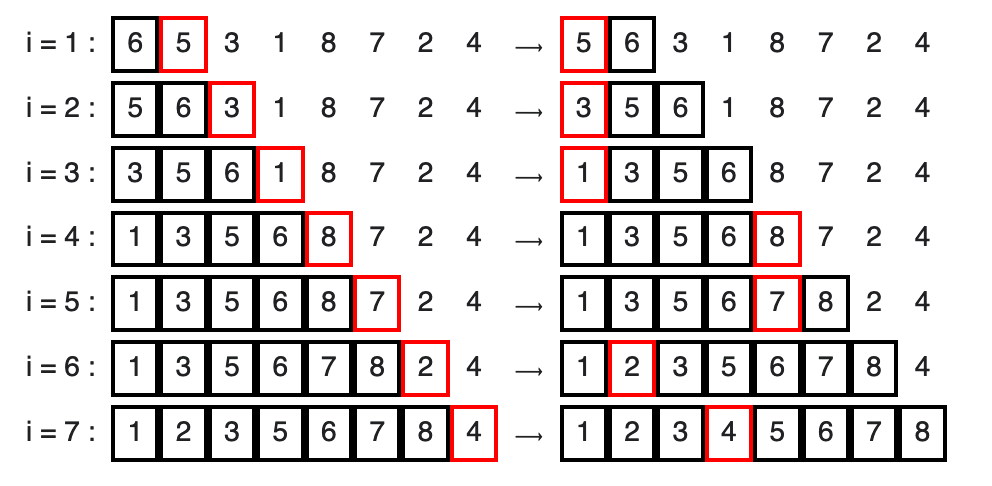
\includegraphics[width=10cm]{images/advanced/InsertionSort.png}
    \end{figure}

    \begin{solution}
        \textbf{Python :}
            \lstinputlisting{solutions/advanced/InsertionSort.py} 
    \end{solution}
    \begin{solution}
        \textbf{Java :}
            \lstinputlisting{solutions/advanced/InsertionSort.java}
    \end{solution}

    \begin{solution}
         La complexité de l'algorithme est de $O(n^2)$ car nous utilisons 2 boucles imbriquées. Dans le pire des cas, la boucle intérieure parcourt la liste une fois pour chaque tour de la boucle extérieure.
    \end{solution}
    
\end{Exercice}


\begin{Exercice} [20 minutes] \textbf{Tri fusion (Merge Sort) - Java} \\
    À partir de deux listes triées, on peut facilement construire une liste triée comportant les éléments issus de ces deux listes (leur \textit{fusion}). Le principe de l'algorithme de tri fusion repose sur cette observation : le plus petit élément de la liste à construire est soit le plus petit élément de la première liste, soit le plus petit élément de la deuxième liste. Ainsi, on peut construire la liste élément par élément en retirant tantôt le premier élément de la première liste, tantôt le premier élément de la deuxième liste (en fait, le plus petit des deux, à supposer qu'aucune des deux listes ne soit vide, sinon la réponse est immédiate). 
    
    Les étapes à suivre pour implémenter l'algorithme sont les suivantes:
    \begin{enumerate}
        \item Si le tableau n'a qu'un élément, il est déjà trié.
        \item Sinon, séparer le tableau en deux parties plus ou moins égales.
        \item Trier récursivement les deux parties avec l'algorithme de tri fusion.
        \item Fusionner les deux tableaux triés en un seul tableau trié.
    \end{enumerate}
    
    Soit la liste \lstinline{l} suivante [38, 27, 43, 3, 9, 82, 10], triez les éléments de la liste en utilisant un tri fusion. Combien d'itération effectuez-vous?
    
    \begin{itemize}
        \item \textbf{Java :}
            \lstinputlisting{code/advanced/MergeSort.java}
    \end{itemize}
    
    \begin{conseil}
    \begin{itemize}
        \item L'algorithme est récursif. 
        \item Revenez à la visualisation de l'algorithme dans les diapositives du cours pour comprendre comment marche concrètement le tri fusion. 
    \end{itemize}
    
    \end{conseil}
    
     \begin{solution}
        \textbf{Java :}
        \lstinputlisting[language=java, firstline=1, firstnumber = 1, lastline=20]{solutions/advanced/MergeSort.java}
    \end{solution}
    \begin{solution}
        \lstinputlisting[language=java, firstline=21, firstnumber = 21]{solutions/advanced/MergeSort.java}
    \end{solution}
    \begin{solution}
        
        Le tri fusion est un algorithme récursif. Ainsi, nous pouvons exprimer sa complexité temporelle via une relation de récurrence : $T(n) = 2T(n/2) + O(n)$. En effet, l'algorithme comporte 3 étapes :
        \begin{enumerate}
            \item ``Divide Step'', qui divise les listes en deux sous-listes, et cela prend un temps constant
            \item ``Conquer Step'', qui trie récursivement les sous-listes de taille $n/2$ chacune, et cette étape est représentée par le terme $2T(n/2)$ dans l'équation.
            \item La dernière étape consiste à fusionner les listes, sa complexité est de $O(n)$.
        \end{enumerate}
        La solution à cette équation est $O(n \log n)$.
    \end{solution}
\end{Exercice}

\end{document}



